\documentclass{amsart}
\usepackage{amsmath, amssymb}
\usepackage{tikz-cd}
\usepackage{mathbbol} % mathbb on greek letters

% hyperref
\usepackage[bookmarks=true, linktocpage=true,
bookmarksnumbered=true, breaklinks=true,
pdfstartview=FitH, hyperfigures=false,
plainpages=false, naturalnames=true,
colorlinks=true, pagebackref=true,
pdfpagelabels]{hyperref}
\hypersetup{
	colorlinks,
	citecolor=blue,
	filecolor=blue,
	linkcolor=blue,
	urlcolor=blue
}

% layout
\setlength{\textwidth}{\paperwidth}
\addtolength{\textwidth}{-1.85in}
\setlength{\textheight}{\paperheight}
\addtolength{\textheight}{-2in}
\calclayout

% Updating to MSC2020
\makeatletter
\@namedef{subjclassname@2020}{%
	\textup{2020} Mathematics Subject Classification}
\makeatother

% elements
\renewcommand{\P}{\mathcal{P}}
\renewcommand{\O}{\mathcal{O}}
\renewcommand{\S}{\mathbb{S}}
\newcommand{\A}{\mathcal{A}s}
\newcommand{\M}{\mathcal{M}}

% sets
\newcommand{\Z}{\mathbb{Z}}
\newcommand{\id}{\mathrm{id}}
\newcommand{\End}{\mathrm{End}}
\newcommand{\Hom}{\mathrm{Hom}}
\newcommand{\Bij}{\mathfrak{Bij}}
\newcommand{\G}{\mathfrak{G}}

% categories
\newcommand{\C}{\mathsf{C}}
\newcommand{\Ch}{\mathsf{Mod}}
\newcommand{\Alg}{\mathsf{Alg}}
\newcommand{\coAlg}{\mathsf{coAlg}}
\newcommand{\simplex}{\mathbf{\Delta}}
\newcommand{\sSet}{\mathsf{sSet}}
\newcommand{\cSet}{\mathsf{cSet}}
\newcommand{\Set}{\mathsf{Set}}
\newcommand{\Nec}{\mathsf{Nec}}
\newcommand{\nSet}{\mathsf{nSet}}
\newcommand{\Mon}{\mathsf{Mon}}
\newcommand{\smod}{\mathsf{Mod}_{\S}}
\newcommand{\sbimod}{\mathsf{biMod}_{\S}}
\newcommand{\operads}{\mathsf{Oper}}
\newcommand{\props}{\mathsf{Prop}}

% functors
\DeclareMathOperator*{\tensor}{\otimes}
\newcommand{\chains}{N}
\newcommand{\cochains}{N}
\newcommand{\op}{\mathrm{op}}
\DeclareMathOperator*{\colim}{colim}
\newcommand{\cobar}{\Omega}
\newcommand{\gcobar}{\mathbb{\Omega}}

% environments
\newtheorem{theorem}{Theorem}
\newtheorem{proposition}[theorem]{Proposition}
\newtheorem{lemma}[theorem]{Lemma}
\theoremstyle{definition}
\newtheorem{definition}[theorem]{Definition}
\newtheorem{example}[theorem]{Example}
\newtheorem{remark}[theorem]{Remark}

% other
\newcommand{\anibal}[1]{\textcolor{blue}{\underline{Anibal}: #1}}
\renewcommand{\th}{^\mathrm{th}}

% drawings
\usetikzlibrary{arrows,decorations.markings}
\tikzset{myptr/.style={decoration={markings,mark=at position 1 with %
			{\arrow[scale=2,>=stealth]{>}}},postaction={decorate}}}
		
\newsavebox\preproduct
\begin{lrbox}{\preproduct}
	\begin{tikzpicture}[scale=.3]
	\draw (0,0)--(0,-.8);
	\draw (0,0)--(.5,.5);
	\draw (0,0)--(-.5,.5);
	\end{tikzpicture} 
\end{lrbox}
\newcommand{\product}{% <- this 'right of' is inherited; how to avoid?
	\usebox\preproduct}

\newsavebox\precoproduct
	\begin{lrbox}{\precoproduct}
		\begin{tikzpicture}[scale=.3]
		\draw (0,0)--(0,.8);
		\draw (0,0)--(.5,-.5);
		\draw (0,0)--(-.5,-.5);
		\end{tikzpicture}
	\end{lrbox}
\newcommand{\coproduct}{% <- this 'right of' is inherited; how to avoid?
	\usebox\precoproduct}

\newsavebox\preboundary
\begin{lrbox}{\preboundary}
	\begin{tikzpicture}[scale=.3]
	\draw (0,0)--(0,1.3);
	\draw (.5,0)--(.5,1.3);
	\draw [fill] (0,0) circle [radius=0.1];
	\draw (.9,.6)--(1.3,.6);
	\draw (1.7,0)--(1.7,1.3);
	\draw (2.2,0)--(2.2,1.3);
	\draw [fill] (2.2,0) circle [radius=0.1];
	\end{tikzpicture}
\end{lrbox}
\newcommand{\boundary}{% <- this 'right of' is inherited; how to avoid?
	\usebox\preboundary}

\newsavebox\precoboundary
\begin{lrbox}{\precoboundary}
	\begin{tikzpicture}[scale=.3]
	\draw (0,0)--(0,1.3);
	\draw (.5,0)--(.5,1.3);
	\draw [fill] (0,1.3) circle [radius=0.1];
	\draw (.9,.6)--(1.3,.6);
	\draw (1.7,0)--(1.7,1.3);
	\draw (2.2,0)--(2.2,1.3);
	\draw [fill] (2.2,1.3) circle [radius=0.1];
	\end{tikzpicture}
\end{lrbox}
\newcommand{\coboundary}{% <- this 'right of' is inherited; how to avoid?
	\usebox\precoboundary}

\newsavebox\precounit
\begin{lrbox}{\precounit}
	\begin{tikzpicture}[scale=.3]
	\draw (0,0)--(0,1.3);
	\draw [fill] (0,0) circle [radius=0.1];
	\end{tikzpicture}
\end{lrbox}
\newcommand{\counit}{% <- this 'right of' is inherited; how to avoid?
	\usebox\precounit}

\newsavebox\preidentity
\begin{lrbox}{\preidentity}
	\begin{tikzpicture}[scale=.3]
	\draw (0,0)--(0,1.3);
	\end{tikzpicture}
\end{lrbox}
\newcommand{\identity}{% <- this 'right of' is inherited; how to avoid?
	\usebox\preidentity}

\newsavebox\preunit
\begin{lrbox}{\preunit}
	\begin{tikzpicture}[scale=.3]
	\draw (0,0)--(0,1.3);
	\draw [fill] (0,1.3) circle [radius=0.1];
	\end{tikzpicture}
\end{lrbox}
\newcommand{\unit}{% <- this 'right of' is inherited; how to avoid?
	\usebox\preunit}

\newsavebox\preassociativity
\begin{lrbox}{\preassociativity}
	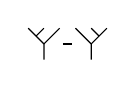
\begin{tikzpicture}[scale=.2]
	\path[draw] (0,0)--(0,1)--(-1,2);
	\draw (0,1)--(1,2);
	\draw (-.5,1.5)--(0,2);
	\draw (1.2,1)--(1.8,1);
	\path[draw] (3,0)--(3,1)--(2,2);
	\draw (3,1)--(4,2);
	\draw (3.5,1.5)--(3,2);	
	\end{tikzpicture}
\end{lrbox}
\newcommand{\associativity}{% <- this 'right of' is inherited; how to avoid?
	\usebox\preassociativity}

\newsavebox\precoassociativity
\begin{lrbox}{\precoassociativity}
	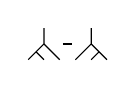
\begin{tikzpicture}[scale=.2]
	\path[draw] (0,0)--(0,-1)--(-1,-2);
	\draw (0,-1)--(1,-2);
	\draw (-.5,-1.5)--(0,-2);
	\draw (1.2,-1)--(1.8,-1);
	\path[draw] (3,0)--(3,-1)--(2,-2);
	\draw (3,-1)--(4,-2);
	\draw (3.5,-1.5)--(3,-2);
	\end{tikzpicture}
\end{lrbox}
\newcommand{\coassociativity}{% <- this 'right of' is inherited; how to avoid?
	\usebox\precoassociativity}

\newsavebox\preinvolution
\begin{lrbox}{\preinvolution}
	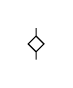
\begin{tikzpicture}[scale=.2]
	\path[draw] (0,0)--(0,.5)--(-.5,1)--(0,1.5)--(0,2);
	\path[draw] (0,.5)--(.5,1)--(0,1.5);
	\end{tikzpicture}
\end{lrbox}
\newcommand{\involution}{% <- this 'right of' is inherited; how to avoid?
	\usebox\preinvolution}

\newsavebox\preleftcounitality
\begin{lrbox}{\preleftcounitality}
	\begin{tikzpicture}[scale=.3]
	\draw (0,0)--(0,.8);
	\draw (0,0)--(.5,-.5);
	\draw (0,0)--(-.5,-.5);
	\draw [fill] (-.5,-.5) circle [radius=0.1];
	\draw (.7,0)--(1.1,0);
	\path[draw] (1.5,-.5)--(1.5,.8);
	\end{tikzpicture}
\end{lrbox}
\newcommand{\leftcounitality}{% <- this 'right of' is inherited; how to avoid?
	\usebox\preleftcounitality}

\newsavebox\preleftcounitcoproduct
\begin{lrbox}{\preleftcounitcoproduct}
	\begin{tikzpicture}[scale=.3]
	\draw (0,0)--(0,.8);
	\draw (0,0)--(.5,-.5);
	\draw (0,0)--(-.5,-.5);
	\draw [fill] (-.5,-.5) circle [radius=0.1];
	\end{tikzpicture}
\end{lrbox}
\newcommand{\leftcounitcoproduct}{% <- this 'right of' is inherited; how to avoid?
	\usebox\preleftcounitcoproduct}

\newsavebox\prerightcounitality
\begin{lrbox}{\prerightcounitality}
	\begin{tikzpicture}[scale=.3]
	\draw (0,0)--(0,.8);
	\draw (0,0)--(.5,-.5);
	\draw (0,0)--(-.5,-.5);
	\draw [fill] (.5,-.5) circle [radius=0.1];
	\draw (-.7,0)--(-1.1,0);
	\path[draw] (-1.5,-.5)--(-1.5,.8);
	\end{tikzpicture}
\end{lrbox}
\newcommand{\rightcounitality}{% <- this 'right of' is inherited; how to avoid?
	\usebox\prerightcounitality}

\newsavebox\prerightcounitcoproduct
\begin{lrbox}{\prerightcounitcoproduct}
	\begin{tikzpicture}[scale=.3]
	\draw (0,0)--(0,.8);
	\draw (0,0)--(.5,-.5);
	\draw (0,0)--(-.5,-.5);
	\draw [fill] (.5,-.5) circle [radius=0.1];
	\end{tikzpicture}
\end{lrbox}
\newcommand{\rightcounitcoproduct}{% <- this 'right of' is inherited; how to avoid?
	\usebox\prerightcounitcoproduct}

\newsavebox\preleftunitality
\begin{lrbox}{\preleftunitality}
	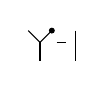
\begin{tikzpicture}[scale=.3]
	\draw (0,0)--(0,-.8);
	\draw (0,0)--(-.5,.5);
	\draw (0,0)--(.5,.5);
	\draw [fill] (.5,.5) circle [radius=0.1];
	\draw (.7,0)--(1.1,0);
	\path[draw] (1.5,.5)--(1.5,-.8);
	\end{tikzpicture}
\end{lrbox}
\newcommand{\leftunitality}{% <- this 'right of' is inherited; how to avoid?
	\usebox\preleftunitality}

\newsavebox\prerightunitality
\begin{lrbox}{\prerightunitality}
	\begin{tikzpicture}[scale=.3]
	\draw (0,0)--(0,-.8);
	\draw (0,0)--(-.5,.5);
	\draw (0,0)--(.5,.5);
	\draw [fill] (-.5,.5) circle [radius=0.1];
	\draw (-.7,0)--(-1.1,0);
	\path[draw] (-1.5,.5)--(-1.5,-.8);
	\end{tikzpicture}
\end{lrbox}
\newcommand{\rightunitality}{% <- this 'right of' is inherited; how to avoid?
	\usebox\prerightunitality}

\newsavebox\preproductcounit
\begin{lrbox}{\preproductcounit}
	\begin{tikzpicture}[scale=.3]
	\draw (0,0)--(0,-.8);
	\draw (0,0)--(.5,.5);
	\draw (0,0)--(-.5,.5);
	\draw [fill] (0,-.8) circle [radius=0.1];
	\end{tikzpicture}
\end{lrbox}
\newcommand{\productcounit}{% <- this 'right of' is inherited; how to avoid?
	\usebox\preproductcounit}

\newsavebox\preunitcoproduct
\begin{lrbox}{\preunitcoproduct}
	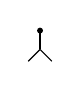
\begin{tikzpicture}[scale=.3]
	\draw (0,0)--(0,.8);
	\draw (0,0)--(.5,-.5);
	\draw (0,0)--(-.5,-.5);
	\draw [fill] (0,.8) circle [radius=0.1];
	\end{tikzpicture}
\end{lrbox}
\newcommand{\unitcoproduct}{% <- this 'right of' is inherited; how to avoid?
	\usebox\preunitcoproduct}

\newsavebox\preleibniz
\begin{lrbox}{\preleibniz}
	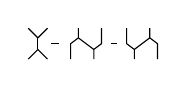
\begin{tikzpicture}[scale=.245]
	\draw (0,.3)--(0,-.3);
	\draw (0,.3)--(.5,.8);
	\draw (0,.3)--(-.5,.8);
	\draw (0,-.3)--(0,.3);
	\draw (0,-.3)--(.5,-.8);
	\draw (0,-.3)--(-.5,-.8);
	
	\draw (.7,0)--(1.1,0);
	\draw (2.1,.8)--(2.1,.3)--(1.7,0)--(1.7,-.8);
	\draw (2.1,.3)--(2.9,-.3);
	\draw (3.3,.8)--(3.3,0)--(2.9,-.3)--(2.9,-.8);
	
	\draw (3.8,0)--(4.1,0);
	\draw (4.6,.8)--(4.6,0)--(5,-.3)--(5,-.8);
	\draw (5,-.3)--(5.8,.3);
	\draw (5.8,.8)--(5.8,.3)--(6.2,0)--(6.2,-.8);	
	\end{tikzpicture}
\end{lrbox}
\newcommand{\leibniz}{% <- this 'right of' is inherited; how to avoid?
	\usebox\preleibniz}

\newsavebox\prebialgebra
\begin{lrbox}{\prebialgebra}
	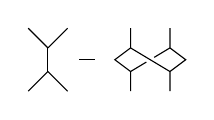
\begin{tikzpicture}[scale=.5]
	\draw (0,.3)--(0,-.3);
	\draw (0,.3)--(.5,.8);
	\draw (0,.3)--(-.5,.8);
	\draw (0,-.3)--(0,.3);
	\draw (0,-.3)--(.5,-.8);
	\draw (0,-.3)--(-.5,-.8);
	
	\draw (.8,0)--(1.2,0);
	
	\draw (2.1,.8)--(2.1,.3)--(1.7,0)--(2.1,-.3)--(2.1,-.8);
	
	\draw (3.1,.8)--(3.1,.3)--(3.5,0)--(3.1,-.3)--(3.1,-.8);

	\draw (2.1,.3)--(3.1,-.3);
	\draw (2.1,-.3)--(2.5,-.06);
	\draw (3.1,.3)--(2.7,.06);	
	\end{tikzpicture}
\end{lrbox}
\newcommand{\bialgebra}{% <- this 'right of' is inherited; how to avoid?
	\usebox\prebialgebra}

\newsavebox\precommutativity
\begin{lrbox}{\precommutativity}
	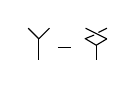
\begin{tikzpicture}[scale=.27]
	\draw (.3,0)--(.3,-1);
	\draw (.3,0)--(.8,.5);
	\draw (.3,0)--(-.2,.5);
	
	\draw (1.2,-.4)--(1.8,-.4);
	
	\draw (3,-.3)--(3,-1);
	\draw (2.5,0)--(3,-.3);
	\draw (3.5,0)--(3,-.3);
	\draw (2.46,0)--(2.9,.18);
	\draw (3.1,.3)--(3.5,.5);
	\draw (3.5,0)--(2.5,.5);
		\end{tikzpicture} 
	\end{lrbox}
	\newcommand{\commutativity}{% <- this 'right of' is inherited; how to avoid?
		\usebox\precommutativity}	

\begin{document}
\title{The cobar construction as an $E_\infty$-Hopf algebra}
\author{Anibal M. Medina-Mardones}
\address{Max Plank Institute for Mathematics, Bonn, Germany}
\email{ammedmar@mpim-bonn.mpg.de}
\address{Department of Mathematics, University of Notre Dame, Notre Dame, IN, USA}
\email{amedinam@nd.edu}
\author{Your name}
\address{Your address}
\email{Your email}

\keywords{.}
\subjclass[2020]{.}

\begin{abstract}
	
\end{abstract} 

\vspace*{-1cm}

\maketitle
\tableofcontents
% !TEX root = ../cobar1.tex

\section{Introduction}

For any topological space $\fX$, its complex of simplicial or cubical singular chains $\Schains(\fX)$ -- regarded as a differential graded (dg) abelian group -- encodes the homology of $\fX$ in its quasi-isomorphism type.
More homotopical information can be stored in the quasi-isomorphism type of this chain complex if considered as a (coassociative) coalgebra, which we will denote $\SchainsA(\fX)$, where the coproduct comes from a natural choice of chain approximation to the diagonal $\fX \to \fX \times \fX$.
For instance, the cohomology ring of $\fX$ is retained, but the action of the Steenrod algebra on its mod~$p$ cohomology is not.

In Mandell's seminal work \cite{mandell2006homotopy_type} it is shown that, when $\fX$ is nilpotent and finite type, the entire homotopy type of $\fX$ can be encoded in the quasi-isomorphism type of this complex if considered as an $E_\infty$-coalgebra, a structure providing $\SchainsA(\fX)$ with coherent homotopies witnessing the derived cocommutativity of the coproduct coming from the strict symmetry of the diagonal map.

The first contribution of this paper is to explicitly endow the cubical singular chains of the based loop space $\loops_x \fX$, with the structure of a monoidal $E_\infty$-coalgebra extending the Serre diagonal.
More specifically, we verify that the monoid structure induced on $\cSchains(\loops_x \fX)$ by the concatenation of loops is compatible with a natural $E_\infty$-coalgebra structure on cubical singular chains, similar to the one defined in \cite{medina2022cube_einfty}.

Applying Adams' cobar construction to the coalgebra of simplicial singular chains of $(\fX, x)$, one obtains another monoidal algebraic model $\cobar \sSchainsA(\fX, x)$ of $\loops_x \fX$ \cite{adams1956cobar}.
More precisely, Adams constructed a natural monoidal chain map $\theta$ from $\cobar \sSchainsA(\fX, x)$ to $\cSchains(\loops_x \fX)$ and proved it to be a quasi-isomorphism if $\fX$ is simply-connected, a statement that also holds true for path-connected spaces after \cite{rivera2018cubical}.
The model $\cobar \sSchainsA(\fX, x)$ is smaller than $\cSchains(\loops_x \fX)$ and unlocks effective analysis of quantitative and qualitative properties of $\loops_x \fX$, as illustrated for instance in \cite{chainalgebraloops} and \cite{adamscobarequivalence}.

The second main contribution of this paper is to make Adams model into a monoidal $E_\infty$-coalgebra and to prove that
\[
\theta \colon \cobar \sSchainsA(\fX, x) \to \cSchains(\loops_x \fX)
\]
respects this higher structure.
Although not pursued in the present article, we remark that the explicit nature of our $E_\infty$-extension invites the study of primary and secondary operations for loops spaces using Adams' model and the tools developed in \cite{medina2021may_st}, \cite{medina2020cartan}, \cite{medina2021adem}, and \cite{medina2021comch}.

Our starting point is groundbreaking work by Baues, which imply statements similar to those in this work but in the category of (coassociative) coalgebras.
Baues reinterpreted Adams' algebraic construction at a deeper geometric level \cite{baues1998hopf}, which allowed him to endow $\cobar \sSchainsA(\fX, x)$ with the structure of a monoidal coalgebra, and to show that $\theta$ preserves this structure.
To prove our statement we interpret Adams' construction at an even deeper categorical level.
We interpret Baues' geometric cobar construction, originally defined for $1$-reduced simplicial sets, as a functor
\begin{equation*}
	\ccobar \colon \sSet^0 \to \Mon_{\cSet},
\end{equation*}
from the category of $0$-reduced simplicial sets to that of monoidal cubical sets.
The key difference with Baues' original work is the use of connections to obtain a natural construction before geometric realization.

Additionally, we need a suitable model of the $E_\infty$-operad endowing cubical chains with a natural $E_\infty$-coalgebra extending the Serre diagonal.
For this we take the operad $\UM$ introduced in \cite{medina2020prop1}.
After proving that its coalgebras form a monoidal category, we show that the functor $\cchainsUM \colon \cSet \to \coAlg_\UM$ -- defined in \cite{medina2022cube_einfty} with a different sign convention -- is monoidal.
This allows us to construct the following extension of Adams and Baues' structures.

\begin{theorem*}
	The following diagram commutes up to natural isomorphisms:
	\[
	\begin{tikzcd} [row sep=small]
		& \Mon_{\coAlg_\UM} \arrow[d] \\
		\Mon_{\cSet} \arrow[ru, "\cchainsUM", out=70, in=180, near start] \arrow[r, "\cchainsA"]
		& \Mon_{\coAlg} \arrow[d] \\
		\sSet^0 \arrow[r, "\cobar \schainsA"] \arrow[u, "\ccobar"]
		& \Mon_{\Ch},
	\end{tikzcd}
	\]
	where the unlabeled arrows are forgetful functors.
\end{theorem*}

In the diagram of the above theorem, the arrow from $\sSet^0$ to $\Mon_{\Ch}$ is Adams' cobar construction, the one from $\sSet^0$ to $\Mon_{\coAlg}$ is Baues' enhancement, and the one from $\sSet^0$ to $\Mon_{\coAlg_{\UM}}$ is our lift.
Additionally, we prove the following statement about Adams's map.

\begin{theorem*}
	For any pointed space $(\fX, x)$,
	\[
	\theta \colon \cobar \sSchainsA(\fX, x) \to \cSchains(\loops_x \fX)
	\]
	is a quasi-isomorphism of monoidal $\UM$-coalgebras.
\end{theorem*}

The fact that $\theta$ respects the monoid structure in $\Ch$ was proven by Adams, whereas the compatibility of the monoid structure with the Serre coalgebra structure was established by Baues.
Our contribution is the compatibility of the monoid structure with a full $E_\infty$-coalgebra extension of Serre's coalgebra.
We also remark that, whereas both Adams and Baues worked in the setting where the underlying space is simply connected, the above theorem does not require any connectivity or finiteness hypotheses.

\subsection*{Related work}

Kadeishvili \cite{kadeishvili1999coproducts, kadeishvili2003cupi} explicitly described monoidal cup-$i$ coproducts on $\cobar \schainsA(X)$ extending Baues coalgebra.
Kadeishvili, as Baues, used cubical methods to define these coproducts and to compare them, in the $1$-connected setting, to cup-$i$ coproducts extending the Serre coalgebra structure on the cubical singular chains of the based loop space.
Additionally, there are several papers \cite{smirnov1990iterated, smith1994cobar, smith2000operads, kadeishvili1998iterating} that predict the existence of, but do not construct, an $E_\infty$-structure on the cobar construction on the chains of simply connected simplicial sets.

On the dual side, Fresse \cite{fresse2003hopf} provided the bar construction of an algebra over the surjection operad with the structure of a comonoid in the category of algebras over the Barratt--Eccles operad.
Additionally, in \cite{fresse2010bar} he used a model category structure on reduced operads \cite{berger2003modelcategory, hinich1997homologicalalgebra} to iterate the bar construction on algebras over cofibrant $E_\infty$-operads.

The use of coalgebras instead of algebras allows us to relate the cobar construction to the based loop space directly --via the Adams map-- without imposing restrictions on the underlying homotopy type, as done by Fresse.
Furthermore, by grounding our approach on the cubical perspective at the heart of Adams' and Baues' seminal papers, we are able to preserve the natural monoidal structures when defining our $E_\infty$-enhancements.

\section{Algebraic preliminaries}

Fix a commutative ring with unit $R$. 
We work over the symmetric monoidal category $(\Ch, \otimes, R)$ of chain complexes of $R$-modules.
As usual, we regard the set of $R$-linear maps $\Hom(C, C^\prime)$ between chain complexes as a chain complex.
The $i\th$ suspension functor $s^i \colon \Ch \to \Ch$ is defined on objects by $(s^{i}M)_n= M_{n-i}$.

A \textit{coassociative counital coalgebra} $C=(C, \partial, \Delta, \varepsilon)$ is the data of an object $(C, \partial) \in \Ch$ equipped with maps $\Delta: C \to C \otimes C$ and $\varepsilon: C\to R$ in $\Ch$ satisfying the usual coassociativity and counitality equations, respectively. 

This notion is equivalent to that of a comonoid in the $(\Ch, \otimes, R)$. Denote by $\coAlg$ the category of coassociative counital coalgebra with morphisms being maps that preserve the structure. 

We notice that $(\coAlg, \otimes, R)$ is symmetric monoidal with structure maps:
\begin{center}
\begin{tikzcd}
C \otimes C^\prime \arrow[r, "\Delta \otimes \Delta^\prime"] &
(C \otimes C) \otimes (C^\prime \otimes C^\prime) \arrow[r, "(23)"] &
(C \otimes C^\prime) \otimes (C \otimes C^\prime),
\end{tikzcd} \par
\begin{tikzcd}
C \otimes C^\prime \arrow[r, "\varepsilon \otimes \varepsilon^\prime"] &
R \otimes R \arrow[r, "\cong"] &
R.
\end{tikzcd}
\end{center}

We will denote the category of monoids on a symmetric monoidal category $\C$ by $\Mon_{\C}$.\footnote{Monoids in $\Ch$ and $\coAlg$ are sometimes referred to as differential graded associative unital algebras and bialgebras respectively, but we avoid this terminology.}




\subsection{The cobar construction}

Let $C$ be a coassociative counital coalgebra. A \textit{coaugmentation} is a morphism $\nu: R \to C$ in $\coAlg$, where $R$ is regarded as a coassociative counital coalgebra concentrated on degree $0$ with coproduct determined by $1 \mapsto 1 \otimes 1$. Denote by $\coAlg^*$ the category of coaugmented coassociative counital coalgebras with morphisms being morphisms of counital coalgebras that preserve coaugmentations. 

We recall the definition of the \textit{cobar} functor 
$$\mathbf{\Omega}: \coAlg^* \to \Mon_{\Ch}.$$

Let  $(C, \partial, \Delta, \varepsilon, \nu)  \in \coAlg^*$ where $\nu: R \to C$ is the coaugmentation. Define
$$\mathbf{\Omega}(C, \partial, \Delta, \varepsilon, \nu) := ( T(s^{-1}  \overline{C} ), D, \mu) \in \Mon_{\Ch}$$ where 
\begin{itemize}
\item $\overline{C}=\text{coker}(\nu: R \to C)$
\item $T(s^{-1} \overline{C})= R \oplus \overline{C} \oplus (\overline{C}  \otimes \overline{C} ) \oplus ( \overline{C} \otimes \overline{C} \otimes \overline{C} ) \oplus\cdots $
\item $\mu: T(s^{-1}  \overline{C} )^{\otimes 2} \to T(s^{-1}  \overline{C} ) $ is the free associative unital product given by concatenation of monomials
\item $D: T(s^{-1}  \overline{C} ) \to T(s^{-1}  \overline{C} )$ is the derivation of degree $-1$ determined by extending the linear map $$- s^{-1} \circ \partial \circ s^{+1} + (s^{-1} \otimes s^{-1}) \circ \Delta \circ s^{+1}: s^{-1}\overline{C} \to s^{-1}\overline{C} \oplus (s^{-1}\overline{C} \otimes s^{-1}\overline{C}) \hookrightarrow T(s^{-1}C)$$ as a derivation.
\end{itemize}

The coassociativity of $\Delta$, the compatibility of $\partial$ and $\Delta$, and the fact that $\partial^2 =0$ together imply that $D^2=0$. This construction is clearly functorial with respect to maps in $\coAlg^*$. We will denote $\mathbf{\Omega} (C, \partial, \Delta, \varepsilon, \nu)$ simply by $\mathbf{\Omega}(C)$. 

In this article we are mostly concerned with \textit{connected} coalgebras, namely $C \in \coAlg^*$ which are non-negatively graded and the coaugmentation $\nu: R \to C$ induces an isomorphism of coalgebras $R \cong C_0$. We denote by $\coAlg^0$ the full subcategory of $\coAlg^*$ consisting of connected coalgebras. If $C \in \coAlg^0$, then $\mathbf{\Omega}(C)$ is concentrated on non-negative degrees. 

The cobar construction was originally applied by Adams' to the coalgebra of normalized chains on a $1$-reduced simplicial set to obtain a model for the chains on the based loop space \cite{Adams}. The cobar construction as a model for the based loop space was furthered studied in \cite{Baues} and more recently, in the non-simply connected setting in \cite{Hess-Tonks}, \cite{Rivera-Zeinalian}.


---
Discuss the localized version of the cobar construction. ---
%\section{The prop $\M$}

\subsection{Operads and props} \label{s:operads and props}

Let $\S$ be the category whose objects are the natural numbers and whose set of morphisms between $m$ and $n$ is empty if $m \neq n$ and is otherwise the symmetric group $\S_n$.
A \textit{left $\S$-module} (resp. \textit{right} $\S$-\textit{module} or $\S$-\textit{bimodule}) is a covariant functor from $\S$ (resp. $\S^\op$ or $\S \times \S^\op$) to $\Ch$.
In this paper we prioritize left module structures over their right counterparts. As usual, taking inverses makes both perspectives equivalent.
We respectively denote by $\smod$ and $\sbimod$ the categories of left $\S$-modules and of $\S$-bimodules with morphisms given by natural transformations.

The collections of group homomorphism $\S_n \to \S_n \times \S_1$ for $n \geq 0$ induces a forgetful functor $U \colon \sbimod \to \smod$.
The similarly defined forgetful functor to right $\S$-modules will not be used.

Given an object $C$ in $\C$ define:
\begin{align*}
\End^C(r) &= \Hom(C, C^{\otimes r}),
&\End^C_C(r, s) &= \Hom(C^{\otimes r}, C^{\otimes s}),
\end{align*}
with their natural structures of $\S$-module and $\S$-bimodule respectively.
The forgetful functor $U$ sends $\End^C_C$ to $\End^C$.

We can define \textit{operads} and \textit{props} by enriching $\S$-modules and \mbox{$\S$-bimodules} with certain composition structures.
For a complete presentation of these concepts we refer to Definition 11 and 54 of \cite{Markl08}.
Intuitively, operads and props can be understood by abstracting the composition structure naturally present in the left $\S$-module $\End^C$, naturally an operad, and the $\S$-bimodule $\End^C_C$, naturally a prop.
We remark that the structure on a prop $\P$ restricts to an operad structure on $U(\P)$.

We can also think of operads and props as algebras over the monad associated to the free-forgetful adjunctions
\begin{equation*}
\begin{tikzcd}
\smod \arrow[r, bend left] & \arrow[l, bend left] \operads 
& \text{and} &
\sbimod \arrow[r, bend left] & \arrow[l, bend left] \props
\end{tikzcd}
\end{equation*}
which we now review, see \cite{Markl08} or \cite{Fresse2010props} for a more detailed presentation.

The \textit{free prop} $F(M)$ generated by an \mbox{$\S$-bimodule} $M$ is constructed using open directed graphs with no directed loops that are enriched with a labeling described next. We think of each directed edge as built from two compatibly directed half-edges. For each vertex $v$ of a directed graph $G$, we have the sets $in(v)$ and $out(v)$ of half-edges that are respectively incoming to and outgoing from $v$. Half-edges that do not belong to $in(v)$ or $out(v)$ for any $v$ are divided into the disjoint sets $in(G)$ and $out(G)$ of incoming and outgoing external half-edges. For any positive integer $n$ let $\overline{n} = \{1,\dots,n\}$ and set $\overline{0} = \emptyset$. For any finite set $S$, denote the cardinality of $S$ by $|S|$. The labeling is given by bijections  
\begin{equation*}
\overline{|in(G)|}\to in(G), \qquad
\overline{|out(G)|}\to out(G),
\end{equation*}
and
\begin{equation*}
\overline{|in(v)|}\to in(v), \qquad
\overline{|out(v)|}\to out(v),
\end{equation*}
for every vertex $v$.
We refer to the isomorphism classes of such labeled directed graphs with no directed loops as $(n,m)$\textit{-graphs} denoting the set of these by $\G(m,n)$.
We use graphs immersed in the plane to represent elements in $\G(m,n)$, please see Figure \ref{f:immersion}.
We consider the right action of $\S_n$ and the left action of $\S_m$ on a $(n,m)$-graph given respectively by permuting the labels of $in(G)$ and $out(G)$. This action defines the $\S$-bimodule structure on the free prop
\begin{equation} \label{e:free prop}
F(M)(m,n) \ = \bigoplus_{\Gamma \in \G(m,n)} \bigotimes_{v \in Vert(\Gamma)} out(v) \otimes_{\S_q} M(p, q) \otimes_{\S_p} in(v),
\end{equation}
where we simplified the notation writing $p$ and $q$ for $\overline{|in(v)|}$ and $\overline{|out(v)|}$ respectively. The composition structure is defined by (relabeled) grafting and disjoint union.
The free operad is constructed similarly only using $(1,m)$-graphs.

Let us now focus on the category $\Ch$.
Let $C$ be a chain complex, $\O$ an operad, and $\P$ a prop.
An $\O$-\textit{coalgebra} (resp. $\O$-\textit{algebra} or $\P$-\textit{bialgebra}) structure on $C$ is a structure preserving morphism $\O \to \End^C$ (resp. $\P \to \End_C^C$).

An $\S$-module $M$ is said to be $E_\infty$ if for each $r$ the chain complex $M(r)$ is an algebraic model for the universal bundle $E\S_r$, i.e., it is free as an $\S_r$-module and its homology is that of a point.
An operad is said to be $E_\infty$ if its underlying $\S$-modules is $E_\infty$.
A prop $\P$ is said to be $E_\infty$ if $U(\P)$ is an $E_\infty$ operad.

\begin{figure}
	\begin{tikzpicture}[scale=.6]
\draw (1,3.7) to (1,3); 

\draw (1,3) to [out=205, in=90] (0,0);

\draw [shorten >= 0cm] (.6,2.73) to [out=-100, in=90] (2,0);

\draw [shorten >= .15cm] (1,3) to [out=-25, in=30, distance=1.1cm] (1,1.5);
\draw [shorten <= .1cm] (1,1.5) to [out=210, in=20] (0,1);

\node at (1,3.9){};
\node at (0,-.32){};
\node at (2,-.32){};

\node at (3,1.5){$\sim$\ \ \ };
\end{tikzpicture}
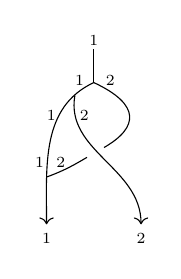
\begin{tikzpicture}[scale=.6]
\draw (1,3.7) to (1,3); 

\draw [->](1,3) to [out=205, in=90] (0,0);

\draw [shorten >= 0cm,->] (.6,2.73) to [out=-100, in=90] (2,0);

\draw [shorten >= .15cm] (1,3) to [out=-25, in=30, distance=1.1cm] (1,1.5);
\draw [shorten <= .1cm] (1,1.5) to [out=210, in=20] (0,1);


\def\x{.8}

\node[scale=\x] at (1,3.9){$\scriptstyle 1$};

\node[scale=\x] at (.7,3.05){$\scriptstyle 1$};
\node[scale=\x] at (1.35,3.05){$\scriptstyle 2$};

\node[scale=\x] at (.1,2.3){$\scriptstyle 1$};
\node[scale=\x] at (.8,2.3){$\scriptstyle 2$};

\node[scale=\x] at (-.15,1.3){$\scriptstyle 1$};
\node[scale=\x] at (.3,1.3){$\scriptstyle 2$};

\node[scale=\x] at (0,-.3){$\scriptstyle 1$};
\node[scale=\x] at (2,-.3){$\scriptstyle 2$};
\end{tikzpicture}
	\caption{Immersed graphs represent labeled directed graphs with the direction implicitly given from top to bottom and the labeling from left to right.}
	\label{f:immersion}
\end{figure}

\subsection{The prop $\M$}

Let us consider the free prop $F(N)$ generated by the $\S$-bimodule $N$ whose only non-zero chain complexes are concentrated in degree $0$ and are give by
\begin{equation*}
N(1, 0)_0 = \Z\{\varepsilon\}, \qquad
N(1, 2)_0 = \Z[\S_2]\{\Delta\}.
\end{equation*}
Define $\A$ as the quotient of $F(N)$ by the prop ideal generated by the relations
\begin{equation*}
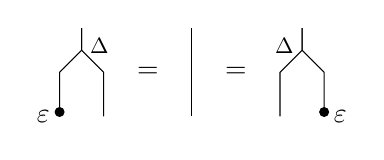
\begin{tikzpicture}[scale=.28]
\draw (-4,0)--(-4,2)--(-5,3)--(-5,4);
\draw (-6,0)--(-6,2)--(-5,3)--(-5,4);
\node [scale=.8] at (-4.2,3.2) {$\Delta$};
\draw [fill] (-6,.2) circle [radius=.2];
\node [left] at (-6,0) {$\varepsilon$};

\node at (-2,2) {=};
\draw (0,0)--(0,4);
\node at (2,2) {=};

\draw (4,0)--(4,2)--(5,3)--(5,4);
\draw (6,0)--(6,2)--(5,3)--(5,4);
\node [scale=.8] at (4.2,3.2) {$\Delta$};
\draw [fill] (6,.2) circle [radius=.2];
\node [right] at (6,0) {$\varepsilon$};
\end{tikzpicture}
\qquad \qquad
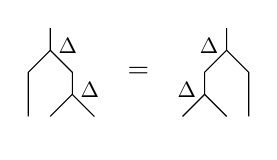
\begin{tikzpicture}[scale=.28]
\node at (0,2){=};
\node at (0,0) {\phantom{$\varepsilon$}};

\draw (2,0)--(3,1)--(3,2)--(4,3)--(4,4);
\draw (4,0)--(3,1);
\draw (4,3)--(5,2)--(5,0);
\node [scale=.8] at (3.2,3.2) {$\Delta$};
\node [scale=.8] at (2.2,1.2) {$\Delta$};

\draw (-2,0)--(-3,1)--(-3,2)--(-4,3)--(-4,4);
\draw (-4,0)--(-3,1);
\draw (-4,3)--(-5,2)--(-5,0);
\node [scale=.8] at (-3.2,3.2) {$\Delta$};
\node [scale=.8] at (-2.2,1.2) {$\Delta$};
\end{tikzpicture}
\end{equation*}
We remark that the category $\coAlg_{U(\A)}$ is equivalent to $\coAlg$.

Let $W^{(1)}$ be the chain complex of free $\Z[\S_2]$-modules
\begin{equation*}
\begin{tikzcd}
\Z[\S_2]\{\nu\} &[0pt] \arrow[l, "1-T"'] \Z[\S_2]\{\mu\},
\end{tikzcd} 
\end{equation*}
which is isomorphic to the cellular chains on the standard $\S_2$-equivariant $CW$-structure on the circle
\begin{equation*}
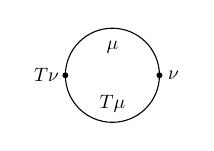
\begin{tikzpicture}[scale=.85]
\draw (0,0) circle (20pt);
\node[scale=.7] at (0,12pt){$\mu$};
\node[scale=.7] at (0,-12pt){$T \mu$};
\node[scale=.7] at (-28pt,0){$T \nu$};
\node[scale=.7] at (26pt,0){$\nu$};
\draw [fill] (-20pt,0) circle [radius=1pt];
\draw [fill] (20pt,0) circle [radius=1pt];
\end{tikzpicture}
\end{equation*}
and let $W^{(0)}$ be the subcomplex generated by $\nu$. We think of $W^{(1)}$ as an $\S_2$-equivariant 1-cell with boundary $W^{(0)}$.

We regard these complexes as $\S$-bimodules concentrated in biarity $(2,1)$, and let $\varphi \colon W^{(0)} \to \A$ be define by sending $T \nu$ and $\nu$ respectively to
\begin{equation*}
\begin{tikzpicture}[scale=.2]
\draw (-4,0)--(-4,4);
\draw (-6,0)--(-6,4);
\draw [fill] (-6,.2) circle [radius=.2];
\node [left] at (-6,0) {$\varepsilon$};

\node at (0,.4) {and};

\draw (4,0)--(4,4);
\draw (6,0)--(6,4);
\draw [fill] (6,.2) circle [radius=.2];
\node [right] at (6,0) {$\varepsilon$.};
\end{tikzpicture}
\end{equation*}
Consider the push-out
\begin{equation*}
\begin{tikzcd}
F(W^{(0)}) \arrow[r, "F(\varphi)"] \arrow[d] & \A \arrow[d, dashed] \\
F(W^{(1)}) \arrow[r, dashed] & \mu \vee_\varphi \A
\end{tikzcd}
\end{equation*}
in the category of props. We think of $\mu \vee_\varphi \A$ as the prop obtained by attaching a $1$-cell in biarity $(2,1)$ to $\A$.

Define $\M$ as the quotient of $\mu \vee_\varphi \A$ by the ideal generated by
\begin{equation*}
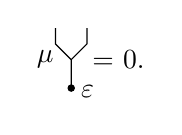
\begin{tikzpicture}[scale=.2]
\draw (5,4)--(5,3)--(6,2)--(6,0);
\draw (7,4)--(7,3)--(6,2);
\node [left] at (5.5,2) {$\mu$};
\draw [fill] (6,.2) circle [radius=.2];
\node [right] at (6,0) {$\varepsilon$};

\node at (9,2) {= 0.};
\end{tikzpicture}
\end{equation*}

We can give a more explicit description of $\M$ using the description of the free prop in terms of $(m,n)$-graphs.
Consider the following elements in $\M$
\begin{equation*}
\counit \in \mathcal M(1,0)_0, \hspace*{.6cm} \coproduct \in \mathcal M(1,2)_0, \hspace*{.6cm} \product \in \mathcal M(2,1)_1,
\end{equation*}
where the decorations by $\varepsilon$, $\Delta$, and $\mu$ are omitted.
Any element in $\M(m,n)$ can be written as a linear combination of the $(m,n)$-graphs generated by these three by grafting, disjoint union and relabeling, modulo the ideals generated by the relations
\begin{equation*}
\qquad \leftcounitality \, , \qquad \rightcounitality \, , \qquad \coassociativity \, , \qquad \productcounit \, .
\end{equation*}
Its chain complex structure is determined using \eqref{e:free prop} by 
\begin{equation*}
\partial\ \counit = 0, \hspace*{.6cm} \partial \ \coproduct = 0, \hspace*{.6cm} \partial \ \product = \ \boundary \, .
\end{equation*}

We have the following results from \cite{Medina20prop1}

\begin{proposition}
	The prop $\M$ is an $E_\infty$-prop.
\end{proposition}

Since $\A$ includes into $\M$, we have that $U(\M)$-coalgebras are $U(\A)$-coalgebras and that there is a functor $\coAlg_{U(\M)} \to \coAlg_{U(\A)}$.


\section{Combinatorial $\M$-bialgebras}

Recall that a category is said to be \textit{small} if its objects and morphisms form sets. A category is said to be \textit{cocomplete} if any functor to it from a small category has a colimit.
If $\mathsf{A}$ is small and $\mathsf{C}$ cocomplete, then the (left) \textit{Kan extension of $g$ along $f$} exists for any pair of functors
\begin{equation*}
\begin{tikzcd}[column sep=small, row sep=small]
\mathsf{A} \arrow[d, "f"'] \arrow[r, "g"] & \mathsf{C} \\ 
\mathsf{B} \arrow[dashed, ur] & \quad .
\end{tikzcd}
\end{equation*}
Given categories $\mathsf{B}$ and $\C$, we denote the \textit{functor category} between them as $\Fun(\mathsf{B}, \C)$.


\subsection{On simplices}

For any non-negative integer $n$ denote by $[n]$ the category generated by the poset (or finite ordinal) $\{0 \to 1 \to \dots \to n\}$.
The \textit{simplex category} $\simplex$ is the category with objects $[0], [1], \dots$ and morphisms given by all functors $f \colon [n] \to [m]$.
The morphisms in $\simplex$ are generated by the usual
\textit{simplicial co-face} and \textit{co-degeneracy maps}
\begin{equation*}
\delta_i \colon [n-1] \to [n], \qquad \sigma_i \colon [n+1] \to [n]
\end{equation*}
for $j \in \{0, \dots, n\}$.
We denote by $\simplex_{\deg}$ the subcategory of $\simplex$ with the same objects and morphisms of the form $\sigma_i \circ \tau$ for any morphism $\tau$ of $\simplex$.

The category of \textit{simplicial sets} is the functor category $\sSet = \Fun(\simplex^\op, \Set)$.
The \textit{standard $n$-simplex} is the simplicial set $\simplex^n = \simplex(-, [n])$, and the \textit{Yoneda embedding} $\Y \colon \simplex \to \sSet$ is the functor induced by $[n] \mapsto \cube^n$.
For any simplicial set $X$ we have
\begin{equation*}
X_n \cong \colim_{\simplex^n \to X} \simplex^n.
\end{equation*}

Consider the functor $\simplex \to \Ch$ defined by
\begin{equation*}
\schains([n])_m = \frac{R\{\simplex([m], [n])\}}{R\{\simplex_{\deg}([m], [n])\}},
\qquad \qquad
\partial(\tau) = \sum (-1)^i \tau \circ \delta_i.
\end{equation*}

We review from \cite{Medina20prop1} a natural $\mathcal M$-bialgebra structure on the normalized chains of standard simplices $\schains(\triangle^n)$.
The $\M$-bialgebra is specified by three linear maps, the images of the generators
\begin{equation*}
\counit, \quad \coproduct, \quad \product,
\end{equation*}
satisfying the relations in the presentation of $\mathcal M$. For $n \in \mathbb{N}$, define: \vspace*{5pt} \\
(1) The counit $\epsilon \in \Hom(\schains(\triangle^n), \Z)$ by
\begin{equation*}
\epsilon \big( [v_0, \dots, v_q] \big) = \begin{cases} 1 & \text{ if } q = 0, \\ 0 & \text{ if } q>0. \end{cases}
\end{equation*}
(2) The coproduct $\Delta \in \Hom(\schains(\triangle^n), \schains(\triangle^n)^{\otimes2})$ by
\begin{equation*}
\Delta \big( [v_0, \dots, v_q] \big) = \sum_{i=0}^q [v_0, \dots, v_i] \otimes [v_i, \dots, v_q].
\end{equation*}
(3) The product $\ast \in \Hom(\schains(\triangle^n)^{\otimes 2}, \schains(\triangle^n))$ by
\begin{equation*}
\left[v_0, \dots, v_p \right] \ast \left[v_{p+1}, \dots, v_q\right] = \begin{cases} (-1)^{p+|\pi|} \left[v_{\pi(0)}, \dots, v_{\pi(q)}\right] & \text{ if } v_i \neq v_j \text{ for } i \neq j, \\
0 & \text{ if not}, \end{cases}
\end{equation*}
where $\pi$ is the permutation that orders the totally ordered set of vertices, and $(-1)^{|\pi|}$ its sign. The coproduct $\Delta$ is known as the \textit{Alexander-Whitney diagonal}.

\begin{proposition}[\cite{Medina20prop1}] \label{p:simplicial chain bialgebra}
	For every $n \in \mathbb{N}$, the assignment
	\begin{equation*}
	\counit \mapsto \epsilon, \quad \coproduct \mapsto \Delta, \quad \product \mapsto \ast,
	\end{equation*}
	defines a natural $\mathcal M$-bialgebra structure  on $\schains(\triangle^n)$.
\end{proposition}

\begin{proof}
	See Theorem 4.2 in \cite{Medina20prop1}.
\end{proof}

 By applying the forgetful functor $U$ from the category of props to the category of operads, the construction of Proposition \ref{p:simplicial chain bialgebra} gives rise to a functor $\simplex \to \coAlg_{U(\M)}$. Since the category of coalgebras over an operad is cocomplete, we may use Kan extension along the Yoneda embedding to define a lift of the functor of chains regarded as a coalgebra with the Alexander-Whitney diagonal:
\begin{equation*}
\begin{tikzcd}[column sep=small, row sep=small]
& \coAlg_{U(\M)} \arrow[d] \\
& \coAlg \arrow[d] \\
\sSet \arrow[r, "N"] \arrow[dashed, uur, bend left]& \Ch.
\end{tikzcd}
\end{equation*}

As explained in \cite{Medina20prop1}, this $E_\infty$-coalgebra on simplicial chains generalizes the constructions of McClure-Smith \cite{McClure-Smith} and Berger-Fresse \cite{Berger-Fresse}.

\subsection{Cubes}

For any positive integer $n$, write $[1]^n$ for the cartesian product of $n$ copies of the category $[1]=\{0 \to 1\}$. We adopt the convention that $[1]^0=[0]$. 

The \textit{cube category with connections} $\square_c$ is the category with objects given by the set $\{[1]^0, [1]^1, [1]^2,...\}$ as objects and whose morphisms are generated by the following three kinds of functors:
\\
\textit{cubical co-face functors} $\delta^{\epsilon}_{j}: [1]^n \to [1]^{n+1}$, where $j=1,...,n+1$, and $\epsilon \in \{0,1\}$, defined by
\begin{eqnarray*}
\delta^{j}_{\epsilon}(t_1,...,t_n)=(t_1,...,t_{j-1},\epsilon,t_j,...,t_n),
\end{eqnarray*}
\textit{cubical co-degeneracy functors} $\varepsilon_{j}: [1]^n \to [1]^{n-1}$, where $j=1,...,n$, defined by
\begin{eqnarray*}
\varepsilon^{j}(t_1,...,t_n)=(t_1,...,t_{j-1},t_{j+1},...,t_n), \text{ and }
\end{eqnarray*}
\textit{cubical co-connection functors} $\gamma_{j}: [1]^n \to [1]^{n-1}$, where $j=1,...,n-1$, $n\geq 2$, defined by
\begin{eqnarray*}
\gamma^{j}(t_1,...,t_n)=(t_1,...,t_{j-1},\text{max}(t_j,t_{j+1}),t_{j+2},...,t_n).
\end{eqnarray*}
A \textit{cubical set with connections} is a functor $C: \square_c^{op} \to \Set.$ Given any cubical set with connections $C$, we will write $C_n= C( [1]^n ), \delta^{\epsilon}_j := C( \delta^{j}_{\epsilon}): C_n \to C_{n-1}, \varepsilon_j=C(\varepsilon^j): C_{n-1} \to C_n$, and $\gamma_j=C(\gamma^j): C_{n-1} \to C_n$, and call $\delta^{\epsilon}_j, \varepsilon_j,$ and $\gamma_j$ the face, degeneracy, and connection maps of $C$, respectively. Cubical sets with connections form a category, denoted by $\cSet$, with morphisms being natural transformations. We denote by $\square_c^n \in \cSet$ the cubical set with connections corepresented by $[1]^n,$ i.e $\square_c^n:= \Hom_{\square_c}(\text{ \_ ,}[1]^n)$. 

\begin{remark} The \textit{cube category} $\square$ is the subcategory of $\square_c$ with the same objects and morphisms generated by cubical co-face and co-degeneracy functors. Cubical sets are usually defined as functors $\square^{op} \to \Set$. However, for this article we will need to include connections maps into our data, so this more standard notion will not be considered. 
\end{remark}




%The \textit{cube category} $\square$ is the free strict monoidal category with a \textit{bipointed object}
%\begin{equation*}
%\begin{tikzcd}
%1 \arrow[r, bend left, "\delta^0"] \arrow[r, bend right, "\delta^1"'] & 2 \arrow[r, "\sigma"] & 1
%\end{tikzcd}
%\end{equation*}
%such that $\sigma \circ \delta^0 = \sigma \circ \delta^1 = \mathrm{id}$. Explicitly, it contains an object $2^n$ for each non-negative integer $n$ and its morphisms are generated by the \textit{coface} and \textit{codegeneracy maps} defined by
%\begin{align*}
%\delta_i^\varepsilon & = \mathrm{id}_{2^{i-1}} \times \delta^\varepsilon \times \mathrm{id}_{2^{n-1-i}} \colon 2^{n-1} \to 2^n, \\
%\sigma_i & = \mathrm{id}_{2^{i-1}} \times \, \sigma \times \mathrm{id}_{2^{n-i}} \colon 2^{n} \to 2^{n-1}.
%\end{align*}

%A \textit{cubical set} $X$ is a contravariant functor from the cube category to the category of sets and a cubical map is a natural transformation between two cubical sets. As is customary, we use the notation
%\begin{equation*}
%X\big( 2^n \big) = X_n \qquad X(\delta^\varepsilon_i) = d^\varepsilon_i \qquad X(\sigma_i) = s_i,
%\end{equation*}
%and refer to elements in the image of any $s_i$ as \textit{degenerate}.

%For each $n \in \mathbb{N}$, the cubical set $\square^n$ is defined by
%\begin{equation*}
%\square^n_k  = \Hom_{\square} \big( 2^k, 2^n \big), \qquad 
%d^\varepsilon_i(x) = x \circ \delta^\varepsilon_i, \qquad 
%s_i(x) = x \circ \sigma_i,
%\end{equation*}
%notice that iteratively
%\begin{equation*}
%\square^n = \overbrace{\square^1 \times \cdots \times \square^1}^{n \text{ times }}.
%\end{equation*}
%We represent the non-degenerate elements of $\square^n$ as sequences $x_1 \cdots\, x_n$ with each $x_i \in \{[0], [1], [0,1]\}$. Any cubical set can be expressed as a colimit of these
%\begin{equation*}
%X \cong \colim_{\square^n \to X} \square^n.
%\end{equation*}



\section{Hopf structures}

By definition, the functor of chains $\cchains \colon \cube \to \Ch$ is monoidal, i.e., the diagram
\begin{equation*}
\begin{tikzcd}
2^p \times 2^q \arrow[r, "\cong"] \arrow[d, "\cchains \otimes \cchains"']& 2^{p+q} \arrow[d, "\cchains"] \\
\cchains(\cube^p) \otimes \cchains(\cube^q) \arrow[r, "\cong"] & \cchains(\cube^{p+q})
\end{tikzcd}
\end{equation*}
commutes and $\cchains(2^0) = R$.
Its lift to the symmetric monoidal category $\coAlg$ is also monoidal since the following diagrams associated to the Serre diagonal and augmentation map commute:
\begin{equation*}
\begin{tikzcd}
\cchains(\cube^p) \otimes \cchains(\cube^{q}) \arrow[r, "\cong"] \arrow[d, "(23) \circ (\Delta \otimes \Delta)"'] & \cchains(\cube^{p+q}) \arrow[d, "\Delta"]\\
\cchains(\cube^p)^{\otimes 2} \otimes \cchains(\cube^{q})^{\otimes 2} \arrow[r, "\cong"]& \cchains(\cube^{p+q})^{\otimes 2}
\end{tikzcd}
\qquad \qquad
\begin{tikzcd}
\cchains(\cube^p) \otimes \cchains(\cube^{q}) \arrow[r, "\cong"] \arrow[d, "(\varepsilon \otimes \varepsilon)"'] & \cchains(\cube^{p+q}) \arrow[d, "\varepsilon"] \\
R \otimes R \arrow[r, "\cong"] & R,
\end{tikzcd}
\end{equation*}
please consult \eqref{e:coalgebras are symmetric monoidal1} and \eqref{e:coalgebras are symmetric monoidal2} for the structure maps of the monoidal product of counital coassociative coalgebras.

In this section we will show that the lift \eqref{e:cubical lift to bialgebras} is also monoidal.
In order to make sense of this statement we first need to describe a monoidal structure on $\M$-bialgebras.

To do so we now make $\M$ into a Hopf prop, that is, a prop over the category $\coAlg$.
Explicitly, we will construct chain maps $\Delta_\M(m,n) \colon \M(m,n) \to \M(m,n) \otimes \M(m,n)$ and $\varepsilon_\M(m,n) \colon \M(m,n) \to R$ for every $(m,n)$ compatible with the prop structure of $\M$ and making each $\M(m,n)$ into a counital coassociative coalgebra.
Then, the structure map of the monoidal product of $\M$-bialgebras is given for any $(m,n)$ by 
\begin{equation*}
\begin{tikzcd} [column sep = small, row sep=large]
\M(m,n) \otimes (C \otimes C^\prime)^{\otimes m} \arrow[r, "\Delta_\M \otimes \id"] & \M(m,n) \otimes \M(m,n) \otimes (C \otimes C^\prime)^{\otimes m} \arrow[dl, out=-150, in=30, "Sh"'] &[-25pt] \\
\big(\M(m,n) \otimes C^{\otimes m}\big) \otimes \big(\M(m,n) \otimes C^{\prime\, \otimes m}\big) \arrow[r] & 
C^{\otimes n} \otimes C^{\prime\, \otimes n} \arrow[r, "Sh"] &[-25pt]
(C \otimes C^\prime)^{\otimes n}.
\end{tikzcd}
\end{equation*}

Intuitively, this diagonal is defined on basis elements in $\M(m,n)_d$ as the sum of the $2^d$ summands obtained from the assignments 

FIGURE

We will need the following observations about the Serre diagonal to define the Hopf structure on $\M$.
There is an action of $\S_n$ on $\cchains(\square^n)$ given by permuting the factors of $\cchains(\square^1)^{\otimes n}$.
The Serre diagonal is equivariant with respect to this action in the following sense.

\begin{lemma} \label{l:serre diagonal invariant}
	Let $T$ be the braiding of $\Ch$.
	The following diagram commutes
	\begin{equation*}
	\begin{tikzcd}
	\cchains(\square^1)^{\otimes 2} \arrow[r, "\Delta"] \arrow[d, "T"] &
	\cchains(\square^1)^{\otimes 2} \otimes \cchains(\square^1)^{\otimes 2} \arrow[d, "T \otimes T"] \\
	\cchains(\square^1)^{\otimes 2} \arrow[r, "\Delta"] &
	\cchains(\square^1)^{\otimes 2} \otimes \cchains(\square^1)^{\otimes 2}.
	\end{tikzcd}
	\end{equation*}
\end{lemma}

\begin{proof}
	This can be proven by a straightforward verification. Conceptually, it holds because $(12)(34)(23) = (23)(13)(24)$ in $\S_4$.
\end{proof}

As can be seen from \eqref{e:free prop}, the $(m,n)$-part of the free prop is defined only up to a choice of total order on the set of vertices of the $(m,n)$-graph involved.

\begin{definition}
	Let $\Gamma \in \G(m,n)$ be a representative of an element in $\M(m,n)$ of degree $d$. A \textit{characteristic map} for $\Gamma$ is the chain map \vspace*{-5pt}
	\begin{equation} \label{e:order chain map}
	\begin{tikzcd}[row sep=tiny, column sep=small]
	\iota_\Gamma \colon \cchains(\square^d) \arrow[r] & \M(m,n) \\
	\qquad {[0,1]}^{\otimes d} \arrow[r, |->] & \Gamma.
	\end{tikzcd}
	\end{equation}
	induced by a choice of total order of the vertices of $\Gamma$.
\end{definition}

Since by Lemma~\ref{l:serre diagonal invariant} the Serre diagonal is equivariant, the following is well-defined.
\begin{definition}
	For any $(m,n)$ the \textit{coproduct} $\Delta_\M(m,n) \colon \M(m,n) \to \M(m,n)^{\otimes 2}$ is defined on a basis element $\Gamma$ by
	\begin{equation} \label{e:diagonal of M}
	\Delta_{\M}(\Gamma) = \iota_\Gamma^{\otimes 2} \circ \Delta \left([0,1]^{\otimes d}\right)
	\end{equation}
	where $\iota_\Gamma$ is a characteristic map of $\Gamma$ and $\Delta$ is the Serre diagonal.
	The \textit{counit} $\varepsilon_\M(m,n) \colon \M(m,n) \to R$ is the chain map whose value on basis elements of degree $0$ is $1$. 
\end{definition}

\begin{theorem}
	The collections of maps $\Delta_\M = \{\Delta_\M(m,n)\}_{m,n \geq 0}$ and $\varepsilon_\M = \{\varepsilon_\M(m,n)\}_{m,n\geq0}$ make $\M$ into a Hopf prop, i.e., a prop over the category $\coAlg$.
\end{theorem}

\begin{proof}
	The collection of maps $\Delta_\M$ compatible with the composition structure on $\M$ since given characteristic maps $\iota_\Gamma$ and $\iota_{\Gamma^\prime}$, then $\iota_\Gamma \otimes \iota_{\Gamma^\prime}$ is a characteristic map of any (vertical or horizontal) composition of $\Gamma$ and $\Gamma^\prime$.
	It respects the relations defining $\M$ since
	\begin{center}
		\begin{tikzcd}
		\leftcounitcoproduct \arrow[r, "\Delta_\M"] \arrow[d, <->] &[-0pt] \leftcounitcoproduct \otimes \leftcounitcoproduct \arrow[d, <->] \\
		\identity \arrow[r, "\Delta_\M"] & \ \, \identity \otimes \identity \, ,
		\end{tikzcd}
		\qquad
		\begin{tikzcd}
		\rightcounitcoproduct \arrow[r, "\Delta_\M"] \arrow[d, <->] &[-0pt] \rightcounitcoproduct \otimes \rightcounitcoproduct \arrow[d, <->] \\
		\identity \arrow[r, "\Delta_\M"] & \ \, \identity \otimes \identity \, ,
		\end{tikzcd}
		\qquad
		\begin{tikzcd}
		\leftcomb \arrow[r, "\Delta_\M"] \arrow[d, <->] &[-0pt] \leftcomb \, \otimes \leftcomb \arrow[d, <->] \\
		\rightcomb \arrow[r, "\Delta_\M"] & \, \rightcomb \, \otimes \rightcomb,
		\end{tikzcd}
		\qquad
		\begin{tikzcd}
		\productcounit \arrow[r, "\Delta_\M"] \arrow[d, <->] &[-0pt] \counit\ \counit \, \otimes \productcounit + \productcounit \otimes \, \counit\ \counit \arrow[d, <->] \\
		0 \arrow[r, "\Delta_\M"] & \ 0.
		\end{tikzcd}
	\end{center}
	It is a chain map since
	\begin{center}
		\begin{tikzcd}
		\counit \arrow[r, "\Delta_\M"] \arrow[d, "\partial"'] &[-0pt] \counit \otimes \counit \arrow[d, "\partial"'] \\
		0 \arrow[r, "\Delta_\M"] & \ \, 0 \, ,
		\end{tikzcd}
		\qquad
		\begin{tikzcd}
		\coproduct \arrow[r, "\Delta_\M"] \arrow[d, "\partial"'] &[-0pt] \coproduct \otimes \coproduct \arrow[d, "\partial"'] \\
		0 \arrow[r, "\Delta_\M"] & \ \, 0 \, ,
		\end{tikzcd}
		\qquad
		\begin{tikzcd}
		\product \arrow[r, "\Delta_\M"] \arrow[d, "\partial"'] &[-0pt] \leftboundary \ \otimes \product + \product \otimes\ \rightboundary \arrow[d, "\partial"'] \\
		\rightboundary \,-\, \leftboundary \arrow[r, "\Delta_\M"] &
		\, \rightboundary \otimes \rightboundary \,-\, \leftboundary \otimes \leftboundary\,.
		\end{tikzcd}
	\end{center}
	The compatibility of the collection of maps $\varepsilon_\M$ is checked similarly and is left to the interested reader.
\end{proof}

\begin{theorem}
	The functor $\cube \to \biAlg_{\M}$ of Theorem~\ref{thm: cubical chain bialgebra} is monoidal.
\end{theorem}

\begin{proof}
	We have already establish that the Serre diagonal and the augmentation map are compatible with the monoidal structure of $\cube$. In diagrammatic terms,
	\begin{equation*}
	\begin{tikzcd}
	\coproduct \otimes \cchains(\cube^{p+q}) \arrow[r, "\Delta_\M \otimes Sh"] \arrow[d] &[20pt]
	\left( \ \coproduct \otimes \coproduct \ \right) \otimes
	\cchains(\cube^{p}) \otimes \cchains(\cube^{q}) \arrow[d] \\
	\cchains(\cube^{p+q})^{\otimes 2} \arrow[r, "Sh"] &
	\cchains(\cube^{p})^{\otimes 2} \otimes \cchains(\cube^{q})^{\otimes 2}
	\end{tikzcd}
	\end{equation*}
	and
	\begin{equation*}
	\begin{tikzcd}
	\counit \ \otimes \cchains(\cube^{p+q}) \arrow[r, "\Delta_\M \otimes Sh"] \arrow[d] &[20pt]
	\left( \ \counit \ \otimes \ \counit \ \right) \otimes
	\cchains(\cube^{p}) \otimes \cchains(\cube^{q}) \arrow[d] \\
	R \arrow[r, "\cong"] &
	R \otimes R
	\end{tikzcd}
	\end{equation*}
	commute.
	We will now show that the following diagram commutes:
	\begin{equation*}
	\begin{tikzcd}
	\product \otimes \cchains(\cube^{p+q})^{\otimes 2} \arrow[d] \arrow[r, "\Delta_\M \otimes Sh"] &[20pt]
	\left(\, \ \leftboundary \ \otimes \product + \product \otimes \ \rightboundary \ \, \right) \otimes \cchains(\cube^{p})^{\otimes 2} \otimes \cchains(\cube^{q})^{\otimes 2} \arrow[d]\\
	\cchains(\cube^{p+q}) \arrow[r, "Sh"] &
	\, \cchains(\cube^{p}) \otimes \cchains(\cube^{q}).
	\end{tikzcd}
	\end{equation*}
	Since this is immediate for $p=0$ or $q=0$ and $\cube$ is generated as a monoidal category by $2^1$, we only need to verify the commutativity of this diagram for $p=q=1$.
	Consider $(x_1 \otimes y_1) \otimes (x_2 \otimes y_2) \in \cchains(\cube^1)^{\otimes 2} \otimes \cchains(\cube^1)^{\otimes 2}$.
	We have
	\begin{equation*}
	\begin{split}
	\big((\id \otimes \varepsilon) \otimes \ast \ + \ \ast \otimes (\varepsilon \otimes \Delta)\big) \ (-1)^{\bars{y_1} \bars{x_2}} \ (x_1 \otimes x_2) \otimes (y_1 \otimes y_2) \ & = \\
	(-1)^{\bars{y_1} \bars{x_2} + \bars{x_1} + \bars{x_2} + \bars{y_1}} \ x_1 \cdot \varepsilon(x_2) \otimes y_1 \ast y_2 \ & + \ 
	(-1)^{\bars{y_1} \bars{x_2} + \bars{x_1}} \ x_1 \ast x_2 \otimes \varepsilon(y_1) \ast y_2.
	\end{split}
	\end{equation*}
	The first summand on the left hand side is non-zero only if $\bars{x_2} = \bars{y_1} = \bars{y_2} = 0$, whereas the second is non-zero only if $\bars{x_1} = \bars{x_2} = \bars{y_1} = 0$, so the above is also equal to
	\begin{equation} \label{e:join is monoidal 1}
	(-1)^{\bars{x_1}} \ x_1 \cdot \varepsilon(x_2) \otimes y_1 \ast y_2 \ + \ 
	x_1 \ast x_2 \otimes \varepsilon(y_1) \ast y_2.
	\end{equation}
	On the other hand,
	\begin{align*}
	(x_1 \otimes y_1) \ast (x_2 \otimes y_2) \ & =\ 
	(-1)^{\bars{x_1} + \bars{y_1}} \ (x_1 \ast x_2) \otimes \varepsilon(y_1) \cdot y_2 \ +\
	(-1)^{\bars{x_1} + \bars{y_1}} \ x_1 \cdot \varepsilon(x_2) \otimes (y_1 \ast y_2) \\ \ & =\ 
	(x_1 \ast x_2) \otimes \varepsilon(y_1) \cdot y_2 \ +\
	(-1)^{\bars{x_1}} \ x_1 \cdot \varepsilon(x_2) \otimes (y_1 \ast y_2),
	\end{align*}
	which is equal to \eqref{e:join is monoidal 1} as claimed.
\end{proof}
\section{A necklical model for the based loop space}

We now describe a cubical model for the based loop space of a reduced simplicial set $X \in \sSet^0$. This particular model has the feature that after taking cubical chains we obtain a dg algebra which is naturally \textit{isomorphic} to the cobar construction on the connected dg coalgebra of simplicial normalized chains $\schains(X)$. We also describe a version of the model which is localized at the $1$-simplices of $X$ and recovers the extended cobar construction defined in \cite{hess2010cobar}. This localization step is required in order to obtain the correct homotopy type of the based loop space in the non-simply connected setting.

The construction of the combinatorial model for the based loop space is best described using necklical sets, a notion related to both simplicial sets and cubical sets with connections. Different approaches to this framework can be found in \cite{baues1998hopf}, \cite{galvez2020hopf}, \cite{dugger2011rigidification}, \cite{rivera2018cubical}, \cite{rivera2018cubical}, among other works. Below we give a self contained exposition suitable for our purposes. 




%\subsection{Necklaces} For any ordered sequence of positive integers $(n_1,...,n_k)$ we denote by $\Delta^{n_1} \vee...\vee \Delta^{n_k} \in \sSet$ the simplicial set obtained by identifying the last vertex of $\Delta^{n_i}$ with the first vertex of $\Delta^{n_{i+1}}.$ A simplicial set of the form $T=\Delta^{n_1} \vee...\vee \Delta^{n_k}$, for $n_i>0$ if $k>1$ and $n_i \geq 0$ if $k=1$, is called a \textit{necklace}. For any necklace $T= \Delta^{n_1} \vee...\vee \Delta^{n_k}$ we call each $\Delta^{n_i}$ the \textit{$i$-th bead} of $T$. The set $V_T=T_0$ will be called the \textit{vertices} of the necklace $T$. We denote by $J_T$ to be the subset of $V_T$ consisting of those vertices which are the first or final vertex of some bead; the elements of $J_T$ are called \textit{joints}. For any necklace $T$, the ordering of the vertices of each bead together with the ordering of the beads of $T$ induces a total ordering on $T_0.$ We denote the first and last vertices of $T$ by $\alpha_T$ and $\omega_T$, respectively. The \textit{dimension} of a necklace $T=\Delta^{n_1} \vee...\vee \Delta^{n_k}$ is defined to be $\text{dim}(T)=n_1 + ... +n_k-k.$

%Necklaces form a category $\Nec$ with morphisms being maps of simplicial sets $f: T \to T'$ that preserve the first and last vertices, i.e. satisfying $f(\alpha_T)=\alpha_{T'}$ and $f(\omega_T)=\omega_{T'}.$ A \textit{neckilcal set} is a functor $K: \Nec^{op} \to \Set.$ Necklical sets form a category, denoted by $\nSet$, with morphisms being natural transformations. Denote by $$Y: \Nec \to \nSet$$ the Yoneda embedding, namely the functor given by $\mathcal{Y}(T)(T')= \text{Hom}_{\Nec}(T',T)$ for any $T,T' \in \Nec.$

%The category of necklical sets $\nSet$ is a (non-symmetric) monoidal category when equipped with monoidal structure $\otimes\colon \Nec \times \Nec \to \Nec$ given by $$K \otimes K' = \colim_{\mathcal{Y}(T) \to K, Y(T')\to K'} Y(T \vee T').$$

%We recall Proposition 3.1 of \cite{Rivera and Zeinalian, cubical rigidification}, which describes a set of generators for the morphisms in $\Nec.$

%\begin{proposition}\label{Necmorphs} Any non-identity morphism in $\Nec$ is a composition of morphisms of the following type
%\begin{item}
%\item (i)  $f: T \to T'$ is an injective morphism of necklaces and $ \text{dim}(T')- \text{dim}(T)=1$
%\\
%\item (ii) $f: \Delta^{n_1} \vee ... \vee \Delta^{n_k} \to \Delta^{m_1} \vee ... \vee \Delta^{m_k}$ is a morphism of necklaces of the form $f=f_1 \vee ... \vee f_k$ such that for exactly one $p \in \{1,...,k\}$, $m_p=n_p-1$ and $f_p= s^j: \Delta^{n_p} \to \Delta^{m_p}= \Delta^{n_p-1}$ is a codegeneracy morphism for some $j \in \{0,...,n_p-1\}$, and for all $i \neq p$, $n_i=m_i$ and $f_i=id_{\Delta^{n_i}}$. 
%\\
%\item (iii) $f: \Delta^{n_1} \vee ...\vee \Delta^{n_{p-1}} \vee \Delta^1 \vee \Delta^{n_{p+1}} \vee... \vee  \Delta^{n_k} \to \Delta^{n_1} \vee ...\vee \Delta^{n_{p-1}} \vee \Delta^{n_{p+1}} \vee... \vee  \Delta^{n_k}$ is a morphism of necklaces such that $f$ collapses the $p$-th bead $\Delta^1$  in the domain to the last vertex of the $(p-1)$-th bead in the target and the restriction of $f$ to all the other beads is injective. 
%\end{item}
%\end{proposition}

%\begin{remark}\label{cofaces} Let $T= \Delta^{n_1} \vee ... \vee \Delta^{n_k}$ and $T'= \Delta^{m_1}\vee ... \vee \Delta^{m_l}$ be two necklaces such that $\text{dim}(T')-\text{dim}(T)=1$. Morphisms $f: T \to T'$ of type $(i)$ as in the above proposition can be of one of the following forms:
%\begin{item}
%\item $(ia)$ We have $k=l$ and there exists $p \in \{1,...,k\}$ such that $n_p= m_p - 1$ and $n_i = m_i$ for all $i \neq p$. The morphism $f: T\to T'$ is of the form $$f=id_{\Delta^{n_1}} \vee ... \vee id_{\Delta^{n_{p-1}}} \vee \partial^j \vee id_{\Delta^{n_{p+1}}} \vee id_{\Delta^{n_k}},$$ where $\partial^j: \Delta^{m_p-1} \to \Delta^{m_p}$ is the $j$-th coface map for some $j \in \{1,...,m_p-1\}.$ 

%\item $(ib)$ We have $k=l+1$ and there exists $p \in \{1,,...,k\}$ such that $n_p + n_{p+1} = m_p$ and $n_i=m_i$ for all $i \neq p, p+1$. The morphism $f: T \to T'$ is of the form
%$$f=id_{\Delta^{n_1}} \vee ... \vee id_{\Delta^{n_{p-1}}} \vee f_p \vee id_{\Delta^{n_{p+2}}} \vee id_{\Delta^{n_k}},$$
%where $f_p: \Delta^{n_p} \vee \Delta^{n_{p+1}} \to \Delta^{n_p + n_{p+1}}=\Delta^{m_p}$ is an injective map of necklaces. 
%\end{item}
%\end{remark} 

\subsection{Necklaces} We follow section 4.3 of \cite{Imma, Ralph, Andy} to define the category of necklaces. First let $\mathbf{\Delta}_{*,*}$ be the subcategory of $\mathbf{\Delta}$ consisting of objects $\{ [1], [2],...\}$ and morphisms being functors $f: [n] \to [m]$ satisfying $f(0)=0$ and $f(n)=m$. The category $\mathbf{\Delta}_{*,*}$ is a strict monoidal category when equipped with the monoidal structure $[n] \otimes [m]= [n+m]$ given by identifying objects $n \in [n]$ and $0 \in [m]$.

Given any category $\mathcal{C}$ one can generate a free strict monoidal category $\mathcal{F}(\mathcal{C})$ with monoid structure denoted by $\vee$. The  objects of $\mathcal{F}(\mathcal{C})$ are ordered sequences $C_1 \vee ... \vee C_k$ of objects $C_i \in ob(\mathcal{C})$ together with morphisms given by ordered sequences $(f_1 \vee ... \vee f_k): C_1 \vee ... \vee C_k \to C'_1 \vee ... \vee C'_k$ of morphisms $f_i: C_i \to C'_i$ in $\mathcal{C}.$ The monoidal structure $\vee$ is then given by concatenation of sequences and the empty sequence is the identity object. If $\mathcal{C}$ is equipped with a monoidal structure $\otimes: \mathcal{C} \times \mathcal{C} \to C$ we may define a new category $\mathcal{F}(C, \otimes)$ by formally adding morphisms $\Delta_{C,C'}: C \vee C' \to C \otimes C'$, for all objects $C, C' \in \mathcal{C},$ to $\mathcal{F}(\mathcal{C}).$
 
Define the \textit{category of necklaces} $\Nec$ to be the category  $\mathcal{F}(\mathbf{\Delta}_{*,*}, \otimes)$, where $[n] \otimes [m]=[n+m]$, as defined above. More explicitly, the objects of $\Nec$ are ordered sequences $[n_1] \vee ... \vee[n_k]$ and there are four types of generating morphisms in $\Nec$:
\begin{itemize}
\item $id_{[n_1]} \vee ... \vee id_{[n_{i-1}]} \vee \partial^j \vee id_{[n_{i+1}]} \vee ... \vee id_{[n_k]}: [n_1] \vee ...\vee [n_i-1] \vee... \vee [n_k] \to [n_1] \vee ...\vee [n_i] \vee ...\vee [n_k]$
for $j=1,...,n_i-1$
\item $id_{[n_1]} \vee ... \vee id_{[n_{i-1}]} \vee \Delta_{[j],[n_i-j]} \vee id_{[n_{i+2}]} \vee ... \vee id_{[n_k]}: [n_1] \vee ...\vee [j]\vee [n_{i}-j] \vee... \vee [n_k] \to [n_1] \vee ...\vee [n_i] \vee ...\vee [n_k]$ for $j=1,...,n_i-1$
\item $id_{[n_1]} \vee ... \vee id_{[n_{i-1}]} \vee s^j \vee id_{[n_{i+1}]} \vee ... \vee id_{[n_k]}: [n_1] \vee ...\vee [n_i+1] \vee... \vee [n_k] \to [n_1] \vee ...\vee [n_i] \vee ...\vee [n_k]$ for $j=0,...,n_i$ and $n_i>0$, and 
\item $s^0: [1] \to [0]$
\end{itemize}

The objects of $\Nec$ are called \textit{necklaces}. Given any necklace $T=[n_1] \vee ... \vee[n_k]$ in $\Nec$ define the \textit{dimension} of $T$ by $\text{dim}(T)=n_1+ ...+n_k-k$. A \textit{necklical set} is a functor $K: \Nec^{op} \to \Set$. Necklical sets form a category with natural transformations as morphisms, which we denote by $\nSet.$ Any necklace $T=[n_1] \vee ... \vee[n_k] \in \Nec$ gives rise to a simplicial set $\mathcal{S}(T)= \Delta^{n_1} \vee... \vee \Delta^{n_k} \in \sSet$, where the wedge symbol now means we identify the last vertex of $\Delta^{n_i}$ with the first vertex of $\Delta^{n_{i+1}}$ for $i=1,...,k-1$. Any necklace $T \in \Nec$ also gives rise to a necklical set $\mathcal{Y}(T)=\Hom_{\Nec}(\text{ \_ }, T): \Nec^{op} \to \Set$. These constructions give rise to functors 
$$\mathcal{S} \colon \Nec \to \sSet$$
and
$$\mathcal{Y} \colon \Nec \to \nSet,$$ respectively. 

The category of necklical sets $\nSet$ is a (non-symmetric) monoidal category when equipped with monoidal structure $\otimes\colon \nSet \times \nSet \to \nSet$ given by $$K \otimes K' = \colim_{\mathcal{Y}(T) \to K, \mathcal{Y}(T')\to K'} \mathcal{Y}(T \vee T').$$

We now construct a monoidal functor
$$\mathcal{P}: \Nec \to \square_c.$$

If $T= \Delta^0$ we set $\mathcal{P}(\Delta^0)=[0]$ and on any other $T \in \Nec$ we define $\mathcal{P}( T )= [1]^{\text{dim}(T)}$. In order to define $\mathcal{P}$ on morphisms, it is sufficient to consider the following cases.
\begin{itemize}
\item For any $\partial^j: [n] \to [n+1]$ such that $0< j<{n+1}$, define $\mathcal{P}(\partial^j): [1]^{n-1}\to [1]^{n}$ to be the cubical coface functor $\mathcal{P}(f)= \delta_0^{j}.$ 

\item For any $[j] \vee [n+1-j] \to [n+1]$ such that $0<j<n+1$, define $\mathcal{P}(f): [1]^{n-1}\to [1]^{n}$ to be the cubical coface functor $\mathcal{P}(f)=\delta_1^{j}$.

\item We now consider morphisms of the form $s^j: [n+1] \to [n]$ for $n>0$. If $j=0$ or $j=n$, then $\mathcal{P}(f): [1]^n \to [1]^{n-1}$ is defined to be the cubical codegeneracy functor $\mathcal{P}(f)= \varepsilon^{j}.$ If $0<j<n$, then we define $\mathcal{P}(f): [1]^n \to [1]^{n-1}$ to be the cubical coconnection functor $\gamma^{j}.$

\item For $s^0: [1] \to [0]$ we define $\mathcal{P}(s^0): [0] \to [0]$ to be the identity functor $id_{[0]}.$

\end{itemize}
\begin{remark}
The functor $\mathcal{P}$ is neither faithful or full. However, for any necklace $T' \in \Nec$ with $\text{dim}(T')=n+1$ and any cubical coface functor $\delta_{\epsilon}^j: [1]^n \to [1]^{n+1}$ for $0 \leq j \leq n+1$, there exists a unique pair $(T, f: T \hookrightarrow T')$, where $T \in \Nec$ with $\text{dim}(T)=n$ and $f: T \hookrightarrow T'$ is an injective morphism in $\Nec$, such that $\mathcal{P}(f)=\delta_{\epsilon}^j $.
\end{remark}

The functor $\mathcal{P}: \Nec \to \square_c$ induces an adjunction between $\cSet$ and $\nSet$
with right adjoint
$$\mathcal{P}^*: \cSet \to \nSet$$
and left adjoint
$$\mathcal{P}_{!} : \nSet \to \cSet.$$
Given a cubical set with connections $C: \square_c^{op} \to \Set$, we have $$\mathcal{P}^*(C)= C \circ \mathcal{P}^{op}.$$ Given a necklical set $K: \Nec^{op} \to \Set$, we have $$\mathcal{P}_{!}(K)= \colim_{(\mathcal{Y}(T) \to K) \in \mathcal{Y} \downarrow K} \mathcal{P}(T) \cong \colim_{(\mathcal{Y}(T) \to K) \in \mathcal{Y} \downarrow K} \square_c^{\text{dim}(T)}.$$

\subsection{A monoidal necklical set model for the based loop space}
We define a functor 
$$\gcobar \colon \sSet^0 \to \Mon_{\nSet}.$$
For any $0$-reduced simplicial set $X$, the underlying necklical set $\gcobar(X) \colon \Nec^{op} \to \Set$ is given by
$$\gcobar(X) = \colim_{(f \colon \mathcal{S}(T) \to X) \in  \mathcal{S} \downarrow X} \mathcal{Y}(T).$$
The monoidal structure $$\gcobar(X) \otimes \gcobar(X) \to \gcobar(X)$$
is induced by the monoidal structure $\vee: \Nec \times \Nec \to \Nec$ together with the monoidal structure $\otimes: \nSet \times \nSet \to \nSet$ on necklicals sets. More precisely, for any $S, S' \in \Nec$, the product $$\gcobar(X)(S) \otimes \gcobar(X)(S') \to \gcobar(X)(S \vee S')$$ is given by $$[f\colon \mathcal{S}(T) \to X, a] \otimes [f'\colon \mathcal{S}(T') \to X, a'] \mapsto [f \vee g\colon \mathcal{S}(T\vee T') \to X, a \otimes  a'],$$
where $(f\colon \mathcal{S}(T) \to X), (f'\colon \mathcal{S}(T') \to X) \in \mathcal{S} \downarrow X$, $a\in \mathcal{Y}(T)(S)$, and $a'\in \mathcal{Y}(T')(S')$.
We may formally invert all the $1$-simplices of $X$ inside $\gcobar(X)$ to obtain a localized version of $\gcobar$ as follows. Define 
$$\widehat{\gcobar} \colon \sSet^0 \to \Mon_{\nSet}$$
by letting
$$\widehat{\gcobar}(X)= \mathcal{L}_{X_1}\gcobar(X),$$
namely $\widehat{\gcobar}(X)$ is the monoidal necklical set obtained by adding formal inverses for all $f\colon \Delta^1 \to X$ subject to the usual relations. This results in inverting all $(f: \mathcal{S}(T) \to X) \in \mathcal{S} \downarrow X$ such that $\text{dim}(T)=0.$

\begin{remark}
We give a few remarks regarding the functor $\gcobar \colon \sSet^0 \to \Mon_{\nSet}$.
\\
$i)$ We may define a triangulation functor $\mathcal{T} \colon \cSet \to \sSet$ by $$\mathcal{T}(C) = \colim_{\square^n_c \to C} (\Delta^1)^{\times n}.$$
The composition of functors
$$\mathcal{T} \circ \mathcal{P}_! \circ  \gcobar\colon \sSet^0 \to \Mon_{\sSet}$$ coincides with the \textit{rigidification functor} introduced by Cordier and studied by Lurie, Dugger and Spivak in the theory of $\infty$-categories \cite{Rivera-Zeinalian}. The rigidification functor is the left adjoint of the homotopy coherent nerve functor. 
\\
$(ii)$ For any $X \in \sSet^0$, we also obtain a simplicial monoid $\mathcal{T}\mathcal{P}_! \widehat{\gcobar}(X) \in \Mon_{\sSet}$ and the monoid $\pi_0( \mathcal{T}\mathcal{P}_! \widehat{\gcobar}(X))$ has the property of being a group.
\\
$(iii)$ In the case of arbitrary (not necessarily $0$-reduced) simplicial sets, we may extend  $\gcobar$ to a functor
$$\sSet \to \mathsf{Cat}_{\nSet}$$ from the category of simpicial sets to the category of small categories enriched over the monoidal category of necklical sets. Similarly, we may extend $\widehat{\gcobar}$ to obtain combinatorial model for the path category of an arbitrary simplicial set.
\end{remark}

The main feature of the combinatorial model given by $\gcobar(X)$ is that it coincides with the cobar construction after applying the normalized cubical chains functor. 

\begin{proposition}
There is a natural isomorphisms of functors 
$$\cchains \circ \mathcal{P}_! \circ \gcobar \cong \mathbf{\Omega} \circ \chains: \sSet^0 \to \Mon_{\Ch}.$$
\end{proposition}

\begin{proof} 
Denote by $\iota_n \in (\square^n_c)_n$ the top dimensional non-degenerate element of the standard $n$-cube with connections $\square^n_c$. Note that for any $X \in \sSet^0$, we may represent any non-degenerate $n$-cube $\alpha \in (\mathcal{P}_!(\gcobar(X)))_n$ as a pair $\alpha=[\sigma: \mathcal{Y}(T) \to X, \iota_n]$ for some $T=[n_1] \vee ... \vee [n_k] \in \Nec$ with $\text{dim}(T)=n_1+ ...+n_k-k=n.$

To define an algebra map
$$\varphi_X: \cchains(\mathcal{P}_!(\gcobar(X))) \xrightarrow{\cong} \mathbf{\Omega}(\chains(X))$$
it suffices to define it on any generator of the form $\alpha=[\sigma \colon \Delta^{n+1} \to X, \iota_{n}]$, i.e. when $T$ is of the form $T=[n+1]$, for some $n\geq0$. If $n=0$ let $\varphi_X(\alpha)= [\overline{\sigma}]+ 1_R$, where $[\overline{\sigma}] \in s^{-1} \overline{ \chains(X)} \subset \mathbf{\Omega}(\chains(X))$ denotes the (length $1$) generator in the cobar construction of $\chains(X)$ determined by $\sigma \in X_{n+1}$ and $1_R$ denotes the unit of the underlying ring $R$. If $n>0$, we let $\varphi_X(\alpha)=[\overline{\sigma}]$. A straightforward computation yields that this gives rise to a well defined isomorphism of algebras, which is compatible with the differentials, and natural with respect to maps of simplicial sets.  
\end{proof}
In \cite{Hess and Tonks}, a localized version of the cobar construction of the chains on a $0$-reduced simplicial set was introduced. This construction is not quite functorial on $\coAlg$ since it depends on a choice of basis of the degree $1$ $R$-module of the underlying coalgebra. However, one may define a functor $$\widehat{\mathbf{\Omega}}: \sSet^0 \to \Mon_{\Ch}$$
defined by formally inverting the set of cycles $\{ [\overline{\sigma}]+1_R | \sigma \in X_1 \} \subset \mathbf{\Omega}(\chains(X))_0$ in the associative algebra $\mathbf{\Omega}(\chains(X))$. Hess and Tonks showed that there is a natural chain homotopy equivalence of associative algebras $$\widehat{\mathbf{\Omega}}(X)\simeq \chains(GX),$$ where $GX$ denotes the Kan loop group of $X$. As an immediate consequence of our previous result, we obtain the following localized version of the isomorphism.

\begin{corollary}
There is a natural isomorphism of functors
$$\cchains \circ \mathcal{P}_! \circ \widehat{\gcobar} \cong \widehat{\mathbf{\Omega}} :\sSet^0 \to \Mon_{\Ch},$$ where $\widehat{\mathbf{\Omega}}$ denotes the extended cobar construction of \cite{Hess and Tonks}. 
\end{corollary}






\section{Main theorems}

In this section we prove the theorems stated in the introduction. 

\begin{proof}[Proof of Theorem~\ref{t:1st main thm in the intro}]
    Recall Theorem~\ref{t:lift of chains of cSets to UM coalgebras} stating that the normalized cubical chains functor lifts to a functor $\cchains_{U(\M)} \colon \cSet_c \to \coAlg_{U(\M)}$ extending the coassociative coalgebra given by the Serre diagonal construction.
    Theorem~\ref{t:lift chains on cSet to UM coAlg is monoidal} states that this lift is  monoidal with respect to the Day convolution product on $\cSet_c$ and the monoidal structure on $\coAlg_{U(\M)}$ induced by the Hopf structure of $\M$.
    Therefore, there is an induced functor $\Mon_{\cSet_c} \to \Mon_{\coAlg_{U(\M)}}$ between the associated categories of monoids.
    By Proposition \ref{gcobarandcobar}, the functors $\cchains \circ \gcobar \colon \sSet^0 \to \Mon_{\Ch}$ and $\mathcal{F} \colon \sSet^0 \to \Mon_{\Ch}$ are naturally isomorphic.
    Hence, the functor $\Mon_{\cSet_c} \to \Mon_{\coAlg_{U(\M)}}$ provides a lift of $\mathcal{F} \colon \sSet^0 \to \Mon_{\Ch}$ to a functor  $\sSet^0 \to \Mon_{\coAlg_{U(\M)}}$ which factors through $\gcobar,$ as desired.
\end{proof}

\begin{proof}[Proof of Theorem~\ref{t:2nd main thm in the intro}]
Using Corollary \ref{localizedcobar}, a similar argument as above gives the desired lift in the localized case. 
\end{proof}

Before proving Theorem \ref{t:3rd main thm in the intro} we recall some results and constructions. 
Kan constructed a functor $$G\colon \sSet^0 \to \mathsf{sGrp}$$ known as the \textit{Kan loop group functor}, which models the based loop space functor in terms of simplicial sets. More precisely, for any $X \in \sSet^0$, the geometric realization of the Kan loop group $|G(X)|$ is homotopy equivalent, as a topological monoid, to the based loop space $\Omega|X|$ on the geometric realization of $X$ \cite{Berger}. 


The Kan loop group functor has a right adjoint usually denoted by 
$$\overline{W} \colon \mathsf{sGrp} \to \sSet^0,$$ which is a model for the classifying space of a simplicial group. This adjunction induces an equivalence of homotopy theories in the following sense.

\begin{theorem} \label{kan} There exists a model category structure on the category $\mathsf{sGrp}$ of simplicial groups such that 
\begin{itemize}
    \item weak equivalences are those maps simplicial groups whose underlying map of simplicial sets is a weak homotopy equivalence
    \item all objects are fibrant, and
\item the adjunction
$$G \colon \sSet^0 \leftrightarrows \mathsf{sGrp}\colon \overline{W}$$
becomes a Quillen equivalence when $\sSet^0$ is equipped with the Kan-Quillen model category structure.
\end{itemize}
\end{theorem}

 For the definition of the Kan loop group construction as well as a proof of the above statement we refer to \cite{Goerss-Jardine} Chapter VI. 

In a similar vein, D. Dugger and D. Spivak, inspired by the work of J. Lurie,  proved that the adjunction between the rigidification functor $\mathfrak{C} \colon \sSet \to \mathsf{Cat}_{\sSet}$ and the homotopy coherent nerve functor $\mathfrak{N} \colon \mathsf{Cat}_{\sSet} \to \sSet$ yields an equivalence of homotopy theories that model $\infty$-categories \cite{Dugger-Spivak}.

\begin{theorem} \label{joyalbergner} The adjunction $$ \mathfrak{C} \colon \sSet \leftrightarrows \mathsf{Cat}_{\sSet} \colon \mathfrak{N}$$ induces a Quillen equivalence when $\sSet$ is equipped with the Joyal model structure and $\mathsf{Cat}_{\sSet}$ with the Bergner model structure.
\end{theorem}


\begin{remark} The Bergner model structure on $\mathsf{Cat}_{\sSet}$ has as weak equivalences maps of simplicially enriched categories that induce a weak homotopy equivalence between the simplicial sets of morphisms and are essentially surjective after passing to the homotopy categories. Fibrant objects in the Bergner model structure are precisely categories enriched over Kan complexes. On the other hand, fibrant objects in the Joyal model structure on $\sSet$ are precisely quasi-categories and all objects are cofibrant. The weak equivalences are known as \textit{Joyal equivalences} and, based on the above result, we can take them to be maps of simplicial sets that become weak equivalences of simplicially enriched categories after applying $\mathfrak{C}$. The Kan-Quillen model structure is a left Bousfield localization of the Joyal model structure obtained by localizing the single morphism $\Delta^1 \to \Delta^0.$
\end{remark}


The following statement, which is Proposition 2.6.2 in \cite{Hinich}, relates $\overline{W}$ and $\mathfrak{N}$.

\begin{proposition}\label{hinich} There is a natural transformation of functors $$\varphi: \overline{W} \Longrightarrow \mathfrak{N}$$ such that for any simplicial group $C \in \mathsf{sGrp}$, we have a weak equivalence
$$\varphi_C: \overline{W}(C) \xra{\simeq} \mathfrak{N}(C).$$
\end{proposition} 

 Given a simplicial monoid $M$, or equivalently a simplicially enriched category with one object, and a set of morphisms $A$ in $M$ we denote by $\mathcal{L}_A M$ the simplicial monoid obtained by formally inverting the elements of $A$ in $M$ subject to the usual relations. We denote by $\mathcal{L}M$ the simplicial group obtained by formally inverting all morphisms of $M$ (level by level) subject to the usual relations. We now deduce the following relationship between the rigidification functor $\mathfrak{C}$ and the Kan loop group functor $G$.

\begin{proposition} Let $X \in \sSet^0$ be a reduced simplicial set. There are natural weak equivalences of simplicial monoids
$$\mathcal{L}_{X_1} \mathfrak{C}(X) \xra{\simeq} \mathcal{L}\mathfrak{C}(X) \xra{\simeq} G(X).$$
\end{proposition}

\begin{proof}
Since $\mathfrak{C}$ is a left Quillen functor and every $X \in \sSet$ is cofibrant in the Joyal model structure, it follows from Theorem \ref{joyalbergner} that $\mathfrak{C}(X)$ is cofibrant as well. Proposition 9.5 of \cite{Dwyer-Kan} implies that the natural inclusion $\mathcal{L}_{X_1} \mathfrak{C}(X) \to \mathcal{L}\mathfrak{C}(X)$ is a weak equivalence of simplicially enriched categories. 

By Proposition \ref{hinich} we have that for any $X \in \sSet^0$, $\varphi_{G(X)}: \overline{W}(G(X)) \xra{\simeq} \mathfrak{N}(G(X))$ is a weak homotopy equivalence. By Theorem \ref{kan}, we have a weak homotopy equivalence $X \xra{\simeq} \overline{W}(G(X))$ given by the unit of the adjunction. Composing these two maps we obtain a weak homotopy equivalence
$$X \xra{\simeq} \mathfrak{N}(G(X)).$$ 
The Quillen equivalence of Theorem \ref{joyalbergner} localizes to a Quillen equivalence
$$\mathcal{L} \mathfrak{C} \colon \sSet^0 \leftrightarrows \mathsf{sGrp} \colon \mathfrak{N}\iota$$
when $\sSet^0$ is equipped with the Kan-Quillen model structure and $\mathsf{sGrp}$ with the model structure of Theorem \ref{kan}. Here $\iota: \mathsf{sGrp} \to \mathsf{Cat}_{\sSet}$ denotes the natural inclusion functor. It follows that the adjoint of the weak homotopy equivalence $X \xra{\simeq} \mathfrak{N}(G(X))$ is a weak equivalence of simplicial groups
$$\mathcal{L}\mathfrak{C}(X) \xra{\simeq} G(X).$$ 
\end{proof}

We now have all the ingredients to prove Theorem \ref{t:3rd main thm in the intro}.
\begin{proof}[Proof of Theorem ~\ref{t:3rd main thm in the intro}]

We construct a zig-zag of quasi-isomorphisms of $U(\M)$-coalgebras between $\widehat{\gcobar}(X)$ and $\schains (G(X))$.
The triangulation functor $$\mathcal{T}\colon \cSet \to \sSet$$
has a right adjoint $$\mathcal{U}\colon \sSet \to \cSet$$
given by the formula
$$\mathcal{U}(X)_n= \sSet((\Delta^1)^{\times n}, X)$$
together with the obvious induced cubical faces, degeneracies, and connections. For any $C \in \cSet_c$ there are quasi-isomorphisms of $U(\M)$-coalgebras
$$\schains(TC) \xra{\simeq} \cchains(UTC) \xleftarrow{\simeq} \cchains(C).$$

[Insert proof of the above fact: The first is a weak-equivalence of $E_\infty$ algebras by \cite{medina2021cubical}.]

Applying the above to $C= \widehat{\gcobar}(X),$ we obtain that $\schains(T\widehat{\gcobar}(X))$ and $\schains(\widehat{\gcobar}(X)) \cong \widehat{\mathcal{F}}(X)$ are quasi-isomorphic as $U(\M)$-coalgebras. 

By Theorem ?? of \cite{minichello-rivera-zeinalian} it follows that $T\widehat{\gcobar}(X)$, which is naturally isomorphic to $\mathfrak{C}(X)$, is naturally weak homotopy equivalent to $G(X)$ via a map of simplicial monoids $Sz \colon \mathfrak{C}(X) \xra{\simeq} G(X)$ induced by the ``Szczarba operators". By naturality, we have an induced quasi-isomorphism of $U(\M)$-coalgebras
$$\schains(T\widehat{\gcobar}(X)) \xra{\simeq} \schains(G(X)).$$
Therefore, $\widehat{\mathcal{F}}(X) \cong \cchains(\widehat{\gcobar}(X))$ and $\schains(G(X))$ are quasi-isomorphic as $U(\M)$-coalgebras, as desired. 




\end{proof}

\bibliographystyle{alpha} % ieeetr
\bibliography{biblio}

\end{document}